\subsection{Activities}

\subsubsection{STM32 code improvements}
\begin{itemize}
	\item Now using the external SDRAM.
	\item ST's peripheral library did not allow continuous SPI transfers larger than 65535 bytes.
	\begin{itemize}
		\item This was not a problem on low resolutions.
		\item Larger resolutions segmentated a lot and this significantly increases transmission time.
		\item A combination of EXTI+DMA was implemented to allow single-stream SPI transfers of any size.
		\item This required some changes at the signaling protocol.
		\item All this is library-free code (directly modifying the microcontroller's registers).
	\end{itemize}
	\item Found out at the camera's datasheet that it can be overclocked on low resolutions.
	\item The new transmission signaling is shown in figure \ref{fig_start_frame_time}.
	\begin{itemize}
		\item The START and END signals are driven at the same time.
		\item This is because if only one ISR was written the microprocessor would loss the timing.
		\item STM32's EXTI does not differentiate between rising and falling edges if you want to detect both.
		\item Only one Raspberry signal is needed if it is connected to both STM32 pins.
	\end{itemize}
\end{itemize}
\begin{figure}[ht!]
\begin{center}
\scalebox{1.5}{
\begin{tikztimingtable}
	START			& H H 14{L} ;[dotted] 2{L}; 3{L} H H \\
	END			& H H 14{L} ;[dotted] 2{L}; 3{L} H H \\
	CLK			& L L L 13{C} ;[dotted] 2{C}; 3{C} L\\
	MISO			& U U U 18D{Image pixel data} U U\\
\end{tikztimingtable}
}
\caption{Time diagram showing the new communication protocol between the Raspberry and the STM32.}
\label{fig_start_frame_time}
\end{center}
\end{figure}

%%%%%%%%%%%%%%%%%%%%%%%%%%%%%%%%%%%%%%%%%%%%%%%%%%%%%%%%%%%%%%%%%%%%%%

\subsubsection{Computer vision integration}
\begin{itemize}
	\item The integration was finished.
	\item Current software on the Raspberry Pi side does the following:
	\begin{itemize}
		\item Allocates memory to store frames in every processing stage.
		\item Initializes the SPI peripheral.
		\item Signal the STM32 and read a frame from it.
		\item Optionally draws the frame at any processing stage (see figure \ref{fig_line_detection_integration}) using SDL.
		\item Performs Gaussian blurring, Edge detection and Probabilistic Hough Transform.
		\item Discriminates between lines and outputs the angle of the most important one through UART.
		\item All of the above using the laptop's camera (was needed for testing).
	\end{itemize}
\end{itemize}
\begin{figure}[ht!]
\begin{center}
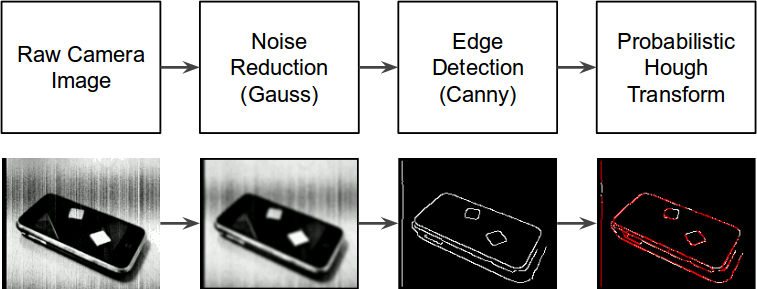
\includegraphics[height=0.35\textwidth]{fig/line_detection_integration}\\
\caption{Steps of line detection running on the Raspberry.}
\label{fig_line_detection_integration}
\end{center}
\end{figure}


%%%%%%%%%%%%%%%%%%%%%%%%%%%%%%%%%%%%%%%%%%%%%%%%%%%%%%%%%%%%%%%%%%%%%%

\subsubsection{Stereo vision depth detection}
\begin{itemize}
	\item This opperation needs to be done on the GPU due to time constraints.
	\begin{itemize}
		\item It is a hevy operation and the CPU could not do it.
		\item An approximate solution needs to be calculated using the GPU.
	\end{itemize}
	\item Raspberry code was started to:
	\begin{itemize}
		\item Initialize, allocate and communicate with the GPU.
		\item Send the camera frames to the GPU.
		\item Perform custom operations on the frames using shaders.
		\item Draw the output.
	\end{itemize}
\end{itemize}
